\scanpage{54}
\mspage{26}
b) $h_1=1$, donc $\dim\operatorname{amb}G=\nu$, on veut $0\leq\nu\leq2$. On voit que le graphe $G$ a au maximum un bout, tous les autres sommets étant donc d'ordre $3$. \deleted{\unsure{Et}} Mais un graphe \inserted{\unsure{top (compact)}} avec $h_1=1$ et n'ayant qu'un seul bout top. est homéom. à
\figure{\begin{tikzpicture}[x=1cm,y=1cm,baseline=-.1cm]
\draw (0,0) .. controls (-1.5,-.8) and (-1.3,1) .. (-.45,.7) .. controls (-.1,.65) and (0,.3) .. (0,0);\draw (0,0)--(1,0.04);\fill (0,0) circle (1.6pt);\fill (1,.04) circle (1.6pt);
\end{tikzpicture}},
et si \deleted{il n'y a pas} \inserted{$G$ n'a pas} de sommets d'ordre $2$, c'est qu'il est \inserted{isom.} au graphe \deleted{\unsure{qui}} combinatoire correspondant à la figure précédente. D'autre part, si le graphe n'a pas de bout, c'est qu'il est homéom. au cercle. Tous ses sommets sont d'ordre $2$, donc de poids marqué $1$, le nb de ces sommets \deleted{de} (il doit être au moins $1$) est \inserted{donc} $1$ \unsure{ou} $2$, ce qui donne
\figure{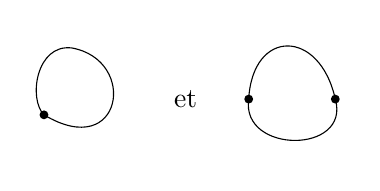
\begin{tikzpicture}[baseline=-.1cm]
\draw (0,0) .. controls (1,-.6) and (1.2,.7) .. (.35,.85) .. controls (-.1,.9) and (-.2,.2) .. (0,0);\fill (0,0) circle (1.6pt);
\node at (1.8,.2) {et};
\draw (2.6,.2) .. controls (2.65,1.1) and (3.5,1.1) .. (3.7,.2) .. controls (3.9,-.5) and (2.5,-.5) .. (2.6,.2);\fill (2.6,.2) circle (1.6pt);\fill (3.7,.2) circle (1.6pt);
\end{tikzpicture}}.
En résumé, on trouve encore trois cas :
\figure{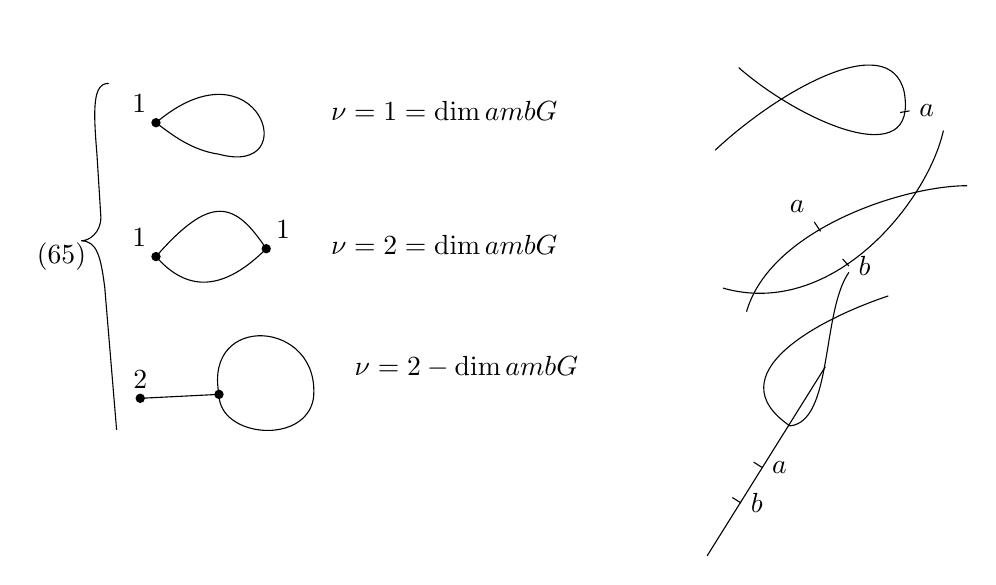
\begin{tikzpicture}[x=1cm,y=1cm]
\node at (-1.2,-1.7) {$(65)$};
\draw (-.6,.5) .. controls (-.8,.5) and (-.8,.2) .. (-.75,-.4) -- (-.7,-1.2) .. controls (-.7,-1.4) and (-.85,-1.5) .. (-.95,-1.5) .. controls (-.75,-1.5) and (-.7,-1.7) .. (-.65,-2.1) -- (-.5,-3.9);
\draw (0,0) .. controls (1.3,1.1) and (1.9,-.7) .. (.8,-.4) .. controls (.45,-.35) and (.2,-.15) .. (0,0);\fill (0,0) circle (1.7pt);\node[above left] at (0,0) {$1$};\node[right] at (2.1,.15) {$\nu=1=\dim\operatorname{amb}G$};
\draw (0,-1.7) .. controls (.7,-.9) and (1,-1) .. (1.4,-1.6) .. controls (.8,-2.2) and (.35,-2.1) .. (0,-1.7);\fill (0,-1.7) circle (1.7pt);\fill (1.4,-1.6) circle (1.7pt);\node[above left] at (0,-1.7) {$1$};\node[above right] at (1.4,-1.6) {$1$};\node[right] at (2.1,-1.55) {$\nu=2=\dim\operatorname{amb}G$};
\draw (-.2,-3.5)--(.8,-3.45);\draw (.8,-3.45) .. controls (.6,-2.4) and (2.1,-2.5) .. (2,-3.5) .. controls (1.9,-4.1) and (.8,-4) .. (.8,-3.45);\fill (-.2,-3.5) circle (1.7pt);\fill (.8,-3.45) circle (1.7pt);\node[above] at (-.2,-3.5) {$2$};\node[right] at (2.4,-3.1) {$\nu=2-\dim\operatorname{amb}G$};
\draw (7.4,.7) .. controls (8.2,0) and (9.7,-.65) .. (9.5,.4) .. controls (9.3,1.2) and (7.9,.4) .. (7.1,-.35);\draw (9.45,.13)--(9.57,.15);\node[right] at (9.57,.15) {$a$};
\draw (7.5,-2.4) .. controls (7.8,-1.35) and (9.5,-.8) .. (10.3,-.8);\draw (7.2,-2.1) .. controls (8.6,-2.5) and (9.8,-1) .. (10,-.1);\draw (8.44,-1.38)--(8.36,-1.26);\node[above left] at (8.36,-1.26) {$a$};\draw (8.72,-1.73)--(8.8,-1.82);\node[right] at (8.8,-1.82) {$b$};
\draw (7,-5.5)--(8.5,-3.1);\draw (8.05,-3.85) .. controls (7.1,-3.2) and (8.4,-2.5) .. (9.3,-2.2);\draw (8.05,-3.85) .. controls (8.6,-3.8) and (8.45,-2.4) .. (8.8,-1.9);\draw (7.7,-4.38)--(7.59,-4.31);\node[right] at (7.7,-4.38) {$a$};\draw (7.43,-4.83)--(7.32,-4.76);\node[right] at (7.43,-4.83) {$b$};
\end{tikzpicture}}
\margin{53}
